% =============================================================================
% IEEE conference-style project report - DBPU (Project 5, Modern Computer Architecture)
% Build:  cd reports && tectonic IEEE_Project_Report.tex     (or: make report)
% All numerical results are copied from analysis/results/summary.md and
% synthesis/SYNTHESIS_RESULTS.md, which are generated by the tool flow.
% =============================================================================
\documentclass[conference]{IEEEtran}
\usepackage{fontspec}
\setmainfont{texgyretermes}[Extension=.otf, UprightFont=*-regular, BoldFont=*-bold, ItalicFont=*-italic, BoldItalicFont=*-bolditalic]
\usepackage{cite}
\usepackage{amsmath,amssymb}
\usepackage{graphicx}
\usepackage{booktabs}
\usepackage{array}
\usepackage{url}
\usepackage[hidelinks]{hyperref}
\graphicspath{{../docs/diagrams/}{../analysis/plots/}{../docs/waveforms/}}
\newcommand{\sig}[1]{\texttt{\detokenize{#1}}}

\begin{document}

\title{Design and Verification of a Dynamic Branch Prediction Unit Using 1-Bit and 2-Bit Saturating Predictors}

\author{
\IEEEauthorblockN{Aaryan Krishna, Pratik Agade, Raghvendra Singh, Vedant Satbhai, Vivek Kumar Raj}
\IEEEauthorblockA{Modern Computer Architecture, Project 5}
}

\maketitle

% -----------------------------------------------------------------------------
\begin{abstract}
Conditional branches create control hazards in pipelined processors: the address of the next
instruction is unknown until the branch is resolved, and every wrong guess forces the pipeline to
discard work. This paper presents the design and verification of a standalone Dynamic Branch
Prediction Unit (DBPU) written in synthesizable Verilog HDL. The unit contains a parameterized
Branch History Table (BHT), interchangeable direction predictors (a static always-not-taken
baseline, a 1-bit last-outcome predictor and a 2-bit saturating-counter predictor), a tagged
direct-mapped Branch Target Buffer (BTB), next-PC selection logic for the fetch stage, and a
misprediction unit that raises a pipeline flush and supplies the corrected PC. The design was
verified with seven self-checking Icarus Verilog testbenches (3282 checks), a pipelined
integration testbench that compares every output against an independent reference model on six
workloads, a row-by-row cross-check of all trace simulations against a Python model, and mutation
testing in which all seven injected bugs were detected. On six synthetic loop-oriented traces fed
identically to all predictors, the 2-bit predictor achieved 81.43\,\% accuracy on a nested loop
(1-bit: 68.57\,\%, static: 15.71\,\%) and 74.38\,\% on a mixed workload (1-bit: 56.25\,\%,
static: 39.38\,\%), lowering the estimated CPI on the mixed workload from 1.242 to 1.103 under a
documented CPI model. Alternating and aliasing patterns are shown to defeat both dynamic
predictors. Yosys synthesis confirms the design is latch-free; mapped to Xilinx 7-series
primitives the 2-bit unit with BTB uses 634 LUTs and 976 flip-flops (pre-place-and-route
estimate).
\end{abstract}

\begin{IEEEkeywords}
branch prediction, control hazard, saturating counter, branch history table, branch target
buffer, pipelining, Verilog HDL, verification
\end{IEEEkeywords}

% -----------------------------------------------------------------------------
\section{Introduction}
Pipelining overlaps the execution of consecutive instructions to raise throughput. In the classic
five-stage pipeline (IF, ID, EX, MEM, WB) a conditional branch such as RISC-V \texttt{BEQ} or
\texttt{BNE}~\cite{waterman2019riscv} is resolved only in EX, two stages after it was fetched.
Until then the fetch stage must guess which instruction comes next. This is a \emph{control
hazard}~\cite{hennessy2017ca,patterson2020cod}. If the guess is wrong, the instructions fetched
on the wrong path are squashed and the cycles spent on them are lost (the misprediction penalty).
Because branches are frequent in real programs, the quality of the guess has a direct effect on
cycles per instruction (CPI).

A \emph{branch predictor} makes this guess in hardware. Static schemes use a fixed rule, such as
``always not taken''. Dynamic schemes learn from the history of each branch at run time. This
project, Project~5 of the Modern Computer Architecture course, implements and compares a static
baseline with the two classic dynamic schemes, the 1-bit and the 2-bit saturating-counter
predictor~\cite{smith1981study}, together with a Branch Target Buffer~\cite{lee1984branch} and a
pipeline flush interface. The objective given in the course specification is to ``design and
evaluate a hardware branch-prediction unit for reducing control-hazard penalties in a pipelined
processor''.

The contributions of this work are: (i) a modular, parameterized and synthesizable Verilog
implementation of the predictors, BHT, BTB, prediction control and misprediction logic;
(ii) a verification environment with self-checking unit tests, a pipelined integration test,
an independent software reference model and mutation testing; and (iii) a reproducible
trace-driven comparison of prediction accuracy and estimated CPI on identical workloads.
The unit is standalone: it exposes a pipeline-style interface but is not embedded in a complete
processor (Section~\ref{sec:conclusion} lists the limitations).

% -----------------------------------------------------------------------------
\section{Literature Review}
\label{sec:lit}
\textbf{Static and early dynamic prediction.} Smith~\cite{smith1981study} studied a range of
strategies on instruction traces, from fixed rules (always taken, predict by opcode, backward
taken/forward not taken) to dynamic schemes that keep per-branch history in a table indexed by
the branch address. That study introduced the use of small saturating counters, showing that a
2-bit counter is more accurate than remembering only the last outcome, because a single atypical
outcome does not immediately reverse the prediction.

\textbf{Branch target buffers.} Knowing the direction is not enough: fetch also needs the target
address before the branch is decoded. Lee and Smith~\cite{lee1984branch} analysed branch target
buffers, caches indexed by the branch address that return the predicted target in the fetch
stage, and their design trade-offs, which makes the BTB a standard companion of a direction
predictor.

\textbf{Two-level and correlating predictors.} Yeh and Patt~\cite{yeh1991two,yeh1993comparison}
proposed two-level adaptive prediction, in which a first level records the history of recent
branch outcomes and a second level of counters is indexed by that history. Pan, So and
Rahmeh~\cite{pan1992improving} showed that the outcome of a branch is correlated with the outcomes
of preceding branches. McFarling~\cite{mcfarling1993combining} combined predictors with a
selector and introduced global-history hashing (gshare), reducing aliasing in the counter tables.

\textbf{Modern predictors.} Later work applied learning to the problem: perceptron
predictors~\cite{jimenez2001dynamic} and the TAGE family, which uses several tagged tables with
geometrically increasing history lengths~\cite{seznec2006case}. Mittal~\cite{mittal2019survey}
surveys these techniques. Textbooks~\cite{hennessy2017ca,patterson2020cod} present the 1-bit and
2-bit BHT, the BTB and the CPI impact of mispredictions as the foundation of this field.

\textbf{Position of this work.} Advanced predictors build on the same basic blocks: a table of
saturating counters, a target buffer and a recovery path. This project implements exactly those
blocks at the register-transfer level and quantifies, on identical inputs, how the counter width
changes accuracy, what aliasing does, and how mispredictions translate into flushes and cycles.

% -----------------------------------------------------------------------------
\section{Problem Statement}
Design, implement in synthesizable Verilog, and verify a hardware branch prediction unit that
(1) predicts the direction of conditional branches (BEQ/BNE) at fetch time using a static
always-not-taken baseline, a dynamic 1-bit predictor and a dynamic 2-bit saturating-counter
predictor; (2) supplies a predicted target through a BTB; (3) learns from the actual outcome
when the branch resolves; (4) detects mispredictions, raises a flush and provides the correct
next PC; and (5) is evaluated on identical loop-oriented branch traces by prediction accuracy,
misprediction rate and estimated CPI, with the three strategies compared fairly.

% -----------------------------------------------------------------------------
\section{Proposed Solution}
\label{sec:solution}
\textbf{Overview.} The DBPU (Fig.~\ref{fig:arch}) is a single top-level module,
\sig{branch_prediction_top}, with an IF-side lookup port and an EX-side resolution port. A
parameter \sig{PREDICTOR_TYPE} selects the direction predictor at elaboration time
(0 static, 1 one-bit, 2 two-bit), so each configuration is real, separately synthesizable
hardware.

\textbf{Predictor design.} The static predictor outputs \emph{not taken} for every PC and has
no storage. The 1-bit predictor stores the last outcome of each BHT entry. The 2-bit predictor
stores a saturating counter per entry with states 00 (strongly not taken), 01 (weakly not taken),
10 (weakly taken) and 11 (strongly taken); the prediction is the most significant bit
(Fig.~\ref{fig:fsm}).

\textbf{BHT organization.} \sig{branch_history_table} is an untagged array of
\sig{ENTRIES} $\times$ \sig{STATE_BITS} registers (default 16 entries). The index is
$\mathit{PC}[\log_2 N + 1 : 2]$, i.e.\ $\mathit{PC}[5{:}2]$ for $N=16$, because instructions are
word aligned. It has two combinational read ports (lookup for IF, read-modify-write for EX) and
one synchronous write port; a synchronous reset loads \sig{INIT_STATE} into every entry
(0 for 1-bit, 01 for 2-bit).

\textbf{Update mechanism.} One parameterized module, \sig{update_logic}, implements an $n$-bit
saturating counter: $+1$ on taken, $-1$ on not taken, holding at the maximum and at zero. With
$n=2$ it realizes the 2-bit table; with $n=1$ it reduces to ``store the last outcome'', so the
same verified logic serves both dynamic predictors.

\textbf{Branch target handling.} \sig{branch_target_buffer} is direct mapped and tagged
(valid bit, tag $\mathit{PC}[31{:}6]$, 32-bit target). It is written only when a branch is
actually taken. \sig{prediction_control} redirects fetch only when the predictor says taken
\emph{and} the BTB hits:
$\mathit{next\_pc} = (\mathit{taken} \wedge \mathit{hit})\ ?\ \mathit{target} : \mathit{PC}+4$.

\textbf{Misprediction detection and flush.} The prediction made in IF travels with the
instruction and returns as \sig{ex_pred_taken} and \sig{ex_pred_next_pc}.
\sig{misprediction_unit} computes the actual next PC and raises
\begin{equation}
\mathit{flush} = \mathit{ex\_valid} \wedge (\mathit{pred\_next\_pc} \neq \mathit{actual\_next\_pc}),
\end{equation}
and provides \sig{ex_correct_pc} $=$ actual next PC. A separate signal \sig{ex_dir_mispredict}
flags direction errors only; it is used for accuracy, while \sig{flush} also captures
``predicted taken but no BTB target'' and stale-target cases.

\begin{figure*}[t]
\centering
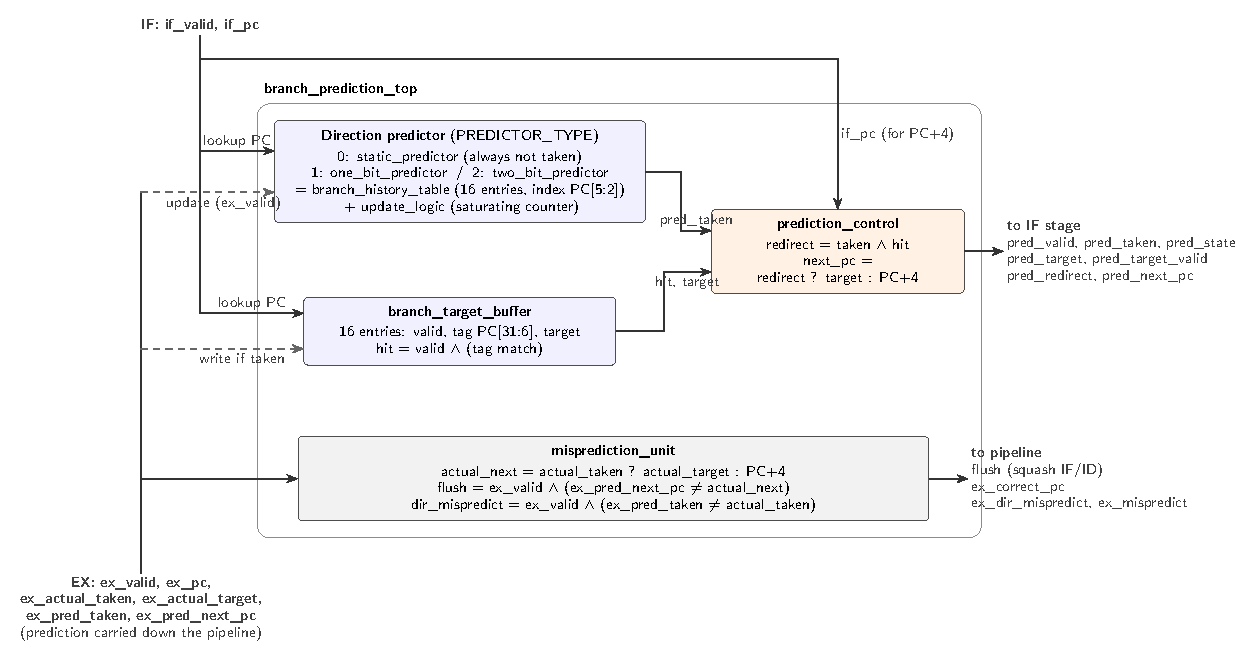
\includegraphics[width=\textwidth]{dbpu_architecture.pdf}
\caption{DBPU architecture as implemented in \texttt{rtl/branch\_prediction\_top.v}. Solid arrows
are combinational paths; dashed arrows are writes performed at the rising clock edge.}
\label{fig:arch}
\end{figure*}

% -----------------------------------------------------------------------------
\section{System Architecture}
Table~\ref{tab:if} lists the interface. On the IF side, \sig{if_valid}/\sig{if_pc} produce the
direction, predictor state, BTB hit and target, and \sig{pred_next_pc} in the same cycle.
On the EX side, \sig{ex_valid} acts as the update enable: at the rising edge the BHT entry of
\sig{ex_pc} is replaced by \sig{update_logic}'s output and, for taken branches, the BTB entry is
written. A lookup of an entry that is being written in the same cycle sees the old value.

\begin{table}[t]
\caption{Top-Level Interface (Widths for \texttt{PC\_WIDTH}=32)}
\label{tab:if}
\centering
\scriptsize
\setlength{\tabcolsep}{3pt}
\begin{tabular}{@{}l c l@{}}
\toprule
Signal & Dir/width & Function \\
\midrule
\sig{if_valid}, \sig{if_pc} & in 1/32 & Lookup request (IF) \\
\sig{pred_taken}, \sig{pred_state} & out 1/2 & Direction, counter state \\
\sig{pred_target_valid}, \sig{pred_target} & out 1/32 & BTB hit, target \\
\sig{pred_redirect}, \sig{pred_next_pc} & out 1/32 & Next fetch address \\
\sig{ex_valid}, \sig{ex_pc} & in 1/32 & Resolve / update \\
\sig{ex_actual_taken}, \sig{ex_actual_target} & in 1/32 & Actual outcome \\
\sig{ex_pred_taken}, \sig{ex_pred_next_pc} & in 1/32 & Prediction from IF \\
\sig{ex_dir_mispredict} & out 1 & Direction was wrong \\
\sig{flush}, \sig{ex_correct_pc} & out 1/32 & Squash, restart address \\
\bottomrule
\end{tabular}
\end{table}

\begin{figure}[t]
\centering
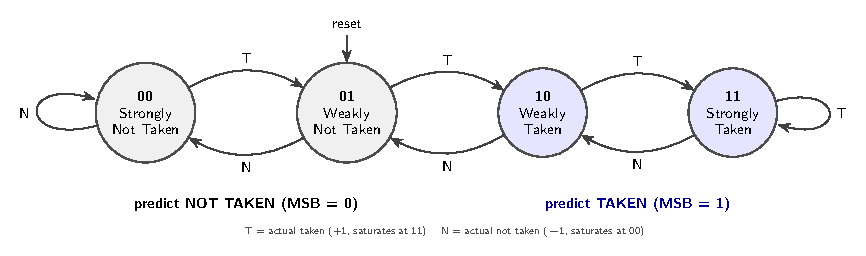
\includegraphics[width=\columnwidth]{two_bit_fsm.pdf}
\caption{2-bit saturating counter implemented by \texttt{update\_logic} (reset state 01).}
\label{fig:fsm}
\end{figure}

% -----------------------------------------------------------------------------
\section{Design Methodology}
The official workflow was followed incrementally: (1) the always-not-taken baseline,
(2) the 1-bit predictor on a parameterized BHT, (3) the 2-bit saturating predictor reusing the
same BHT and update module, (4) the BTB, prediction control and misprediction unit, and
(5) integration. Each step was followed by a unit testbench before moving on.

Tools: Icarus Verilog 13.0~\cite{williams_iverilog} (Verilog-2005~\cite{ieee1364}) for
simulation, Python~3 with Matplotlib for trace generation and analysis, Yosys
0.71~\cite{wolf_yosys} for synthesis, and Git. All steps are scripted in a Makefile
(\texttt{make test}, \texttt{make results}, \texttt{make synth}).

\textbf{Metrics.} For $N$ branches of which $C$ are predicted correctly,
\begin{align}
\text{Accuracy} &= \tfrac{C}{N}\times 100\,\%, \qquad
\text{MR} = \tfrac{N-C}{N},\\
\text{CPI}_{\text{est}} &= \text{CPI}_{\text{base}} + f_b \cdot \text{MR} \cdot P,
\label{eq:cpi}
\end{align}
where MR is the misprediction rate as a fraction, $f_b$ the fraction of instructions that are
branches and $P$ the misprediction penalty. We assume $\text{CPI}_{\text{base}}=1.0$, $f_b=0.20$
and $P=2$ cycles (a branch resolved in EX squashes the instructions in IF and ID). These values
are assumptions, not measurements; they are command-line options of the analysis script.
Speed-up over the baseline is $\text{CPI}_{\text{static}}/\text{CPI}$.

% -----------------------------------------------------------------------------
\section{Verilog Implementation}
Table~\ref{tab:modules} summarises the nine RTL modules. Coding rules: Verilog-2005,
non-blocking assignments in clocked blocks, \texttt{always @(*)} with defaults in combinational
blocks (no latches), synchronous active-high reset for every register, named parameters instead
of magic numbers, and no simulation-only constructs in \texttt{rtl/}. All files compile with
\texttt{iverilog -Wall} without warnings.

\begin{table}[t]
\caption{RTL Modules}
\label{tab:modules}
\centering
\footnotesize
\begin{tabular}{@{}l l@{}}
\toprule
Module & Responsibility \\
\midrule
\sig{branch_prediction_top} & Predictor selection and integration \\
\sig{static_predictor} & Always not taken (baseline) \\
\sig{one_bit_predictor} & 1-bit BHT + update logic \\
\sig{two_bit_predictor} & 2-bit BHT + update logic \\
\sig{branch_history_table} & Untagged table, 2R/1W ports \\
\sig{update_logic} & $n$-bit saturating counter \\
\sig{branch_target_buffer} & Tagged direct-mapped BTB \\
\sig{prediction_control} & IF next-PC selection \\
\sig{misprediction_unit} & EX check, flush, correct PC \\
\bottomrule
\end{tabular}
\end{table}

\textbf{Synthesis.} Yosys elaborated all three configurations, the script asserts that no latch
cells are inferred, and all runs passed. Table~\ref{tab:synth} gives the cell counts after
mapping to Xilinx 7-series primitives (\texttt{synth\_xilinx}). The flip-flop counts match the
expected storage exactly: the BTB holds $16\times(1+26+32)=944$ bits and the BHT 16 or 32 bits.
These are pre-place-and-route estimates; no maximum frequency is reported because no vendor
place-and-route or timing analysis was run, and the design was not implemented on an FPGA board.

\begin{table}[t]
\caption{Yosys Synthesis (Xilinx 7-Series Mapping, 16-Entry BHT/BTB)}
\label{tab:synth}
\centering
\footnotesize
\begin{tabular}{@{}l r r@{}}
\toprule
Configuration & LUTs & Flip-flops \\
\midrule
Static + BTB & 510 & 944 \\
1-bit BHT + BTB & 602 & 960 \\
2-bit BHT + BTB & 634 & 976 \\
1-bit predictor only & 29 & 16 \\
2-bit predictor only & 46 & 32 \\
\bottomrule
\end{tabular}
\end{table}

% -----------------------------------------------------------------------------
\section{Simulation and Verification}
\textbf{Unit tests.} Seven self-checking testbenches compare outputs with expected values and
print a PASS/FAIL verdict (Table~\ref{tab:tests}). They cover reset initialisation of every entry,
the complete 2-bit transition table (checked both on \sig{update_logic} and through the real BHT),
saturation at 11 and 00 with no wrap-around, the loop pattern TTTTTN (1-bit: 2 mispredictions per
loop execution; 2-bit: 1 after warm-up), alternating outcomes (including the effect of the reset state), independent entries, index
aliasing, BHT boundaries and read-during-write, BTB hit/miss/tag-conflict/replacement (including the highest address), and all
misprediction cases, including ``predicted taken but BTB miss''.

\textbf{Pipelined integration.} \sig{tb_branch_prediction_top} runs the three configurations
side by side with five-stage timing: a branch is looked up in IF and resolved in EX two cycles
later, so predictions can see stale state; on \sig{flush} the two younger lookups are squashed
and fetch restarts. Every cycle all ten DUT outputs are compared with a behavioural reference
model, and the cycle count is checked against $N + 2 + 2\times\text{flushes}$. It passed on the
directed stimulus (3013 checks) and on all six traces.

\textbf{Reference-model cross-check and mutation testing.} Every prediction, counter state and
flush logged by the trace simulations was recomputed by an independent Python model: zero
mismatches over 570 branches and twelve BHT-size runs. To show that the tests can actually find
bugs, a script injects one fault at a time into a copy of the RTL (e.g.\ counter wrap-around, BTB
tag check removed, flush on direction error only, wrong index bits); all seven mutants were
detected. Fig.~\ref{fig:wave} is rendered directly from a simulation VCD file.

\begin{table}[t]
\caption{Self-Checking Testbench Results (\texttt{make test})}
\label{tab:tests}
\centering
\footnotesize
\begin{tabular}{@{}l l r@{}}
\toprule
Testbench & Scope & Checks \\
\midrule
\sig{tb_static_predictor} & Test 1 & 83/83 \\
\sig{tb_one_bit_predictor} & Tests 2, 4, 6, 10 & 49/49 \\
\sig{tb_two_bit_predictor} & Tests 3--6, 10 & 70/70 \\
\sig{tb_branch_history_table} & Tests 6, 10 & 33/33 \\
\sig{tb_branch_target_buffer} & Test 11 & 22/22 \\
\sig{tb_misprediction} & Test 9 & 12/12 \\
\sig{tb_branch_prediction_top} & Test 12 & 3013/3013 \\
\bottomrule
\end{tabular}
\end{table}

\begin{figure*}[t]
\centering
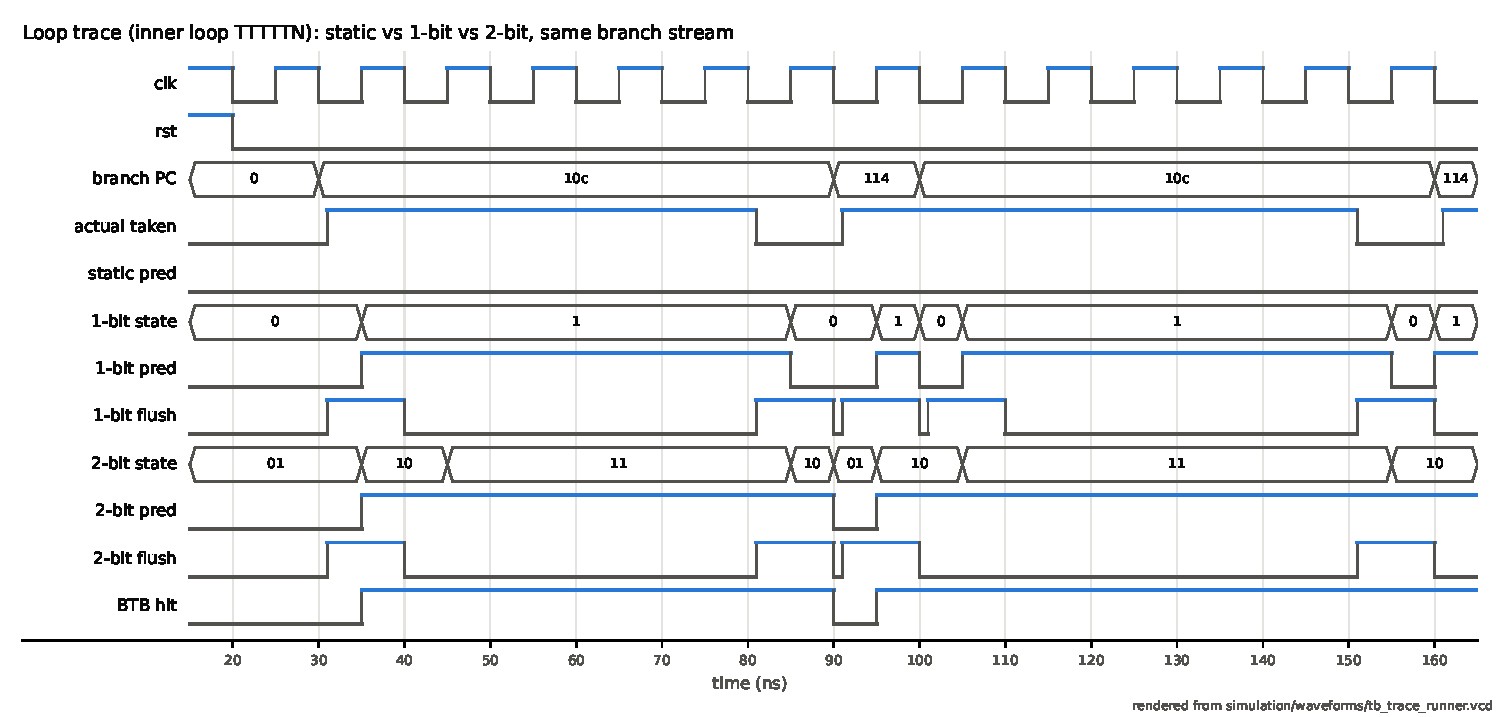
\includegraphics[width=0.92\textwidth]{wave_predictor_comparison.pdf}
\caption{Simulated waveform (loop trace, same branch stream to all predictors). At the loop exit
(80--90\,ns) both dynamic predictors mispredict; the 1-bit state falls to 0 but the 2-bit counter
only to 10, so at the next loop entry (100--110\,ns) only the 1-bit predictor mispredicts again.}
\label{fig:wave}
\end{figure*}

% -----------------------------------------------------------------------------
\section{Performance Evaluation}
Six deterministic traces were generated from small program models (Table~\ref{tab:traces}).
They are synthetic, not captured from a processor. A trace-runner testbench feeds the
\emph{same} trace to three instances of the top module, one branch per cycle with the update
applied before the next lookup (the textbook model), and logs every prediction. The analysis
script computes the metrics of~(\ref{eq:cpi}) from those logs.

\begin{table}[t]
\caption{Branch Workloads}
\label{tab:traces}
\centering
\footnotesize
\begin{tabular}{@{}l r >{\raggedright\arraybackslash}p{4.4cm}@{}}
\toprule
Trace & $N$ & Behaviour \\
\midrule
Loop-heavy & 70 & Nested loop; inner TTTTTN $\times$10, outer back-edge \\
Alternating & 60 & One branch, T N T N \ldots \\
Mostly taken & 100 & 90 T / 10 N, seeded shuffle \\
Mostly not taken & 100 & 10 T / 90 N, seeded shuffle \\
Mixed & 160 & 5 branches: inner loop, data-dependent, rare, alternating, outer loop \\
Aliasing & 80 & Always-T and always-N branch sharing a 16-entry BHT index \\
\bottomrule
\end{tabular}
\end{table}

% -----------------------------------------------------------------------------
\section{Results and Discussion}
Table~\ref{tab:results} and Fig.~\ref{fig:acc} give the results.

\begin{table*}[t]
\caption{Prediction Accuracy and Estimated CPI (16-Entry BHT; CPI Model of Eq.~(\ref{eq:cpi}))}
\label{tab:results}
\centering
\footnotesize
\begin{tabular}{@{}l r rrr rrr rrr@{}}
\toprule
 & & \multicolumn{3}{c}{Mispredictions} & \multicolumn{3}{c}{Accuracy (\%)} & \multicolumn{3}{c}{Estimated CPI} \\
\cmidrule(lr){3-5}\cmidrule(lr){6-8}\cmidrule(l){9-11}
Workload & $N$ & Static & 1-bit & 2-bit & Static & 1-bit & 2-bit & Static & 1-bit & 2-bit \\
\midrule
Loop-heavy       & 70  & 59 & 22 & 13 & 15.71 & 68.57 & \textbf{81.43} & 1.337 & 1.126 & \textbf{1.074} \\
Alternating      & 60  & 30 & 60 & 60 & \textbf{50.00} & 0.00 & 0.00 & \textbf{1.200} & 1.400 & 1.400 \\
Mostly taken     & 100 & 90 & 17 & 13 & 10.00 & 83.00 & \textbf{87.00} & 1.360 & 1.068 & \textbf{1.052} \\
Mostly not taken & 100 & 10 & 18 & 11 & \textbf{90.00} & 82.00 & 89.00 & \textbf{1.040} & 1.072 & 1.044 \\
Mixed            & 160 & 97 & 70 & 41 & 39.38 & 56.25 & \textbf{74.38} & 1.242 & 1.175 & \textbf{1.103} \\
Aliasing         & 80  & 40 & 80 & 80 & \textbf{50.00} & 0.00 & 0.00 & \textbf{1.200} & 1.400 & 1.400 \\
\bottomrule
\end{tabular}
\end{table*}

\begin{figure*}[t]
\centering
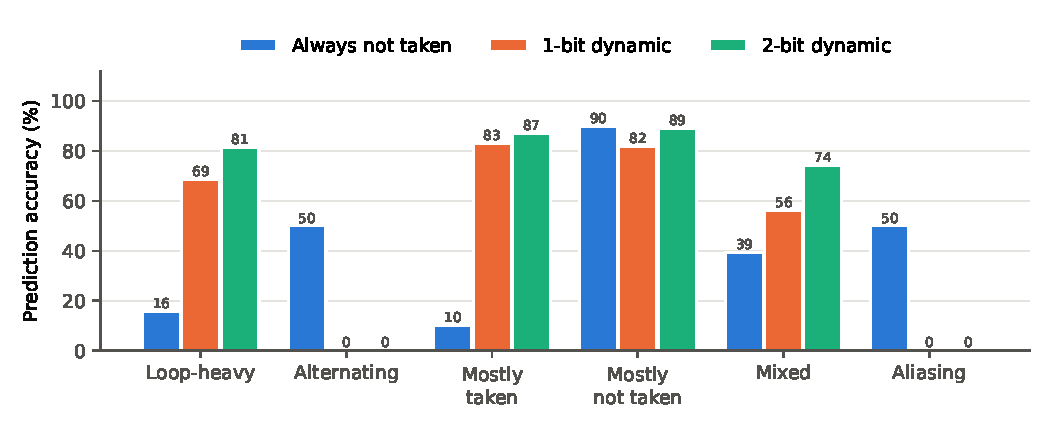
\includegraphics[width=0.78\textwidth]{accuracy_comparison.pdf}
\caption{Direction prediction accuracy of the three predictors on identical traces (RTL simulation).}
\label{fig:acc}
\end{figure*}

\textbf{Loops.} The loop trace confirms the textbook behaviour exactly. The 1-bit predictor
misses twice per inner-loop execution ($2\times10$) plus twice on the outer branch, 22 in total;
the 2-bit predictor misses twice in the first execution and once in each later one, plus twice
on the outer branch, 13 in total. Accuracy rises from 15.71\,\% (static) to 68.57\,\% (1-bit) and
81.43\,\% (2-bit), and the estimated CPI falls from 1.337 to 1.074 (speed-up 1.245).

\textbf{Biased branches.} On the mostly-taken trace both dynamic predictors are far better than
the static one (87\,\% and 83\,\% vs.\ 10\,\%). On the mostly-not-taken trace the static
predictor is already right 90\,\% of the time; the 2-bit predictor nearly matches it (89\,\%),
while the 1-bit predictor drops to 82\,\% because every rare taken branch causes two
mispredictions. The hysteresis of the 2-bit counter limits that damage to one.

\textbf{Pathological patterns.} For strictly alternating outcomes the 1-bit predictor is always
wrong, and the 2-bit predictor, starting at 01, oscillates between 01 and 10 and is also always
wrong, while ``always not taken'' scores 50\,\%. The aliasing trace behaves the same way when its
two opposite branches share one 16-entry BHT entry. A local counter cannot learn such patterns;
history-based predictors~\cite{yeh1991two,pan1992improving,mcfarling1993combining} address them.
Notably, in the aliasing case the tagged BTB prevents the never-taken branch from being
redirected, so in the pipelined run its direction errors cause no flush (60 direction errors but
only 20 flushes).

\textbf{Mixed workload.} With five different branch behaviours the 2-bit predictor achieves
74.38\,\%, 18.1 points above the 1-bit and 35.0 points above the static predictor, and reduces the
estimated CPI from 1.242 to 1.103 (speed-up 1.127).

\textbf{Table size.} Fig.~\ref{fig:sweep} re-runs the RTL with 2 to 64 BHT entries. On the
aliasing trace both dynamic predictors jump from 0\,\% to 98.75\,\% once the table has 32 entries
and the two branches stop sharing an entry. On the mixed trace accuracy saturates at 8 entries.
With only 2 entries the 1-bit predictor happens to score higher than the 2-bit one (63.1\,\% vs.\
51.9\,\%), and with 4 entries the 2-bit predictor scores slightly above its 16-entry value: when
branches share entries, interference can help or hurt, so aliasing effects are workload-specific.

\begin{figure}[t]
\centering
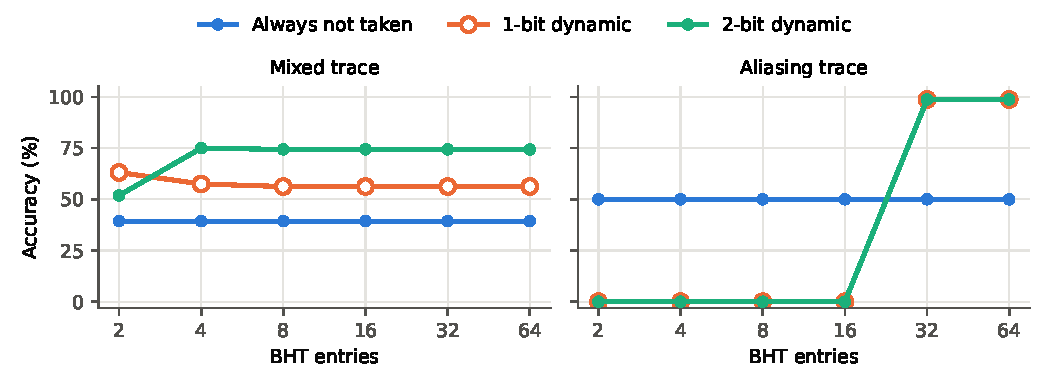
\includegraphics[width=\columnwidth]{bht_size_sweep.pdf}
\caption{Accuracy versus BHT size (RTL recompiled for each size). In the aliasing panel the
1-bit and 2-bit curves coincide.}
\label{fig:sweep}
\end{figure}

\textbf{Pipelined timing.} In the pipelined integration run, where every instruction is a branch
and each flush costs two cycles, the loop trace needed 190, 114 and 96 cycles for the static,
1-bit and 2-bit units (2.71, 1.63 and 1.37 cycles per branch). These cycle counts are measured
from the RTL, but the 100\,\% branch density makes them an upper bound on the penalty rather than
a CPI for real programs.

\textbf{Cost.} The 2-bit predictor alone costs 46 LUTs and 32 flip-flops versus 29 and 16 for the
1-bit predictor (Table~\ref{tab:synth}); with a BTB the BTB dominates the area. The 2-bit counter
therefore buys a clear accuracy gain for a very small amount of extra hardware.

% -----------------------------------------------------------------------------
\section{Individual Contributions}
Table~\ref{tab:contrib} gives each member's area of responsibility. The code and documentation
were developed with the help of an AI assistant (Claude, Anthropic) in sessions directed by the
project coordinator; every member is responsible for reviewing, testing and explaining the parts
they own. The repository commit history and \texttt{docs/CONTRIBUTIONS.md} record the
contributions.

\begin{table}[t]
\caption{Individual Contributions}
\label{tab:contrib}
\centering
\footnotesize
\begin{tabular}{@{}>{\raggedright\arraybackslash}p{2.35cm} >{\raggedright\arraybackslash}p{5.65cm}@{}}
\toprule
Member & Responsibility \\
\midrule
Aaryan Krishna & Coordination, architecture, top-level integration, prediction control and misprediction unit, synthesis, final validation \\
Pratik Agade & Static and 1-bit predictors, Branch Target Buffer \\
Raghvendra Singh & 2-bit predictor, Branch History Table, saturating update logic \\
Vedant Satbhai & Self-checking testbenches, integration test, waveform verification \\
Vivek Kumar Raj & Branch traces, performance analysis, documentation and report integration \\
\bottomrule
\end{tabular}
\end{table}

% -----------------------------------------------------------------------------
\section{Conclusion}
\label{sec:conclusion}
A dynamic branch prediction unit with static, 1-bit and 2-bit direction predictors, a tagged
BTB and a flush interface was implemented in synthesizable Verilog and verified with
self-checking unit and integration testbenches, an independent reference model and mutation
testing. On identical traces the 2-bit saturating counter was the most accurate predictor on
loop-heavy, biased and mixed workloads, at a cost of 17 extra LUTs and 16 extra flip-flops over
the 1-bit predictor, while alternating and aliased branches exposed the limits of local
counters.

\textbf{Limitations.} The unit is standalone and is driven by testbenches that model the IF and
EX stages; it is not integrated into a processor. The traces are synthetic. Only conditional
direct branches are modelled. Synthesis results are pre-place-and-route estimates without
timing, and no FPGA hardware run was performed. The CPI values depend on the stated assumptions.

\textbf{Future work (Phase II).} Integrate the unit into a five-stage RV32I pipeline and measure
real CPI; use traces from compiled benchmarks; add global history (gshare) and a tournament
selector; add return-address prediction; and run place-and-route to obtain timing results.

% -----------------------------------------------------------------------------
\begin{thebibliography}{15}
\bibitem{smith1981study}
J.~E. Smith, ``A study of branch prediction strategies,'' in \emph{Proc. 8th Annu. Symp. Computer
Architecture (ISCA)}, Minneapolis, MN, USA, May 1981, pp. 135--148.

\bibitem{lee1984branch}
J.~K.~F. Lee and A.~J. Smith, ``Branch prediction strategies and branch target buffer design,''
\emph{Computer}, vol.~17, no.~1, pp. 6--22, Jan. 1984, doi: 10.1109/MC.1984.1658927.

\bibitem{yeh1991two}
T.-Y. Yeh and Y.~N. Patt, ``Two-level adaptive training branch prediction,'' in \emph{Proc. 24th
Annu. Int. Symp. Microarchitecture (MICRO-24)}, 1991, pp. 51--61, doi: 10.1145/123465.123475.

\bibitem{yeh1993comparison}
T.-Y. Yeh and Y.~N. Patt, ``A comparison of dynamic branch predictors that use two levels of
branch history,'' in \emph{Proc. 20th Annu. Int. Symp. Computer Architecture (ISCA)}, 1993,
pp. 257--266.

\bibitem{pan1992improving}
S.-T. Pan, K.~So, and J.~T. Rahmeh, ``Improving the accuracy of dynamic branch prediction using
branch correlation,'' in \emph{Proc. 5th Int. Conf. Architectural Support for Programming
Languages and Operating Systems (ASPLOS-V)}, 1992, pp. 76--84, doi: 10.1145/143365.143490.

\bibitem{mcfarling1993combining}
S.~McFarling, ``Combining branch predictors,'' Digital Equipment Corp. Western Research
Laboratory, Palo Alto, CA, USA, Tech. Note TN-36, Jun. 1993.

\bibitem{jimenez2001dynamic}
D.~A. Jim\'enez and C.~Lin, ``Dynamic branch prediction with perceptrons,'' in \emph{Proc. 7th
Int. Symp. High-Performance Computer Architecture (HPCA)}, Monterrey, Mexico, 2001,
pp. 197--206, doi: 10.1109/HPCA.2001.903263.

\bibitem{seznec2006case}
A.~Seznec and P.~Michaud, ``A case for (partially) TAgged GEometric history length branch
prediction,'' \emph{J. Instruction-Level Parallelism}, vol.~8, 2006.

\bibitem{mittal2019survey}
S.~Mittal, ``A survey of techniques for dynamic branch prediction,'' \emph{Concurrency and
Computation: Practice and Experience}, vol.~31, no.~1, 2019, doi: 10.1002/cpe.4666.

\bibitem{hennessy2017ca}
J.~L. Hennessy and D.~A. Patterson, \emph{Computer Architecture: A Quantitative Approach}, 6th~ed.
Cambridge, MA, USA: Morgan Kaufmann, 2017.

\bibitem{patterson2020cod}
D.~A. Patterson and J.~L. Hennessy, \emph{Computer Organization and Design RISC-V Edition: The
Hardware/Software Interface}, 2nd~ed. Cambridge, MA, USA: Morgan Kaufmann, 2020.

\bibitem{waterman2019riscv}
A.~Waterman and K.~Asanovi\'c, Eds., \emph{The RISC-V Instruction Set Manual, Volume I:
Unprivileged ISA}, Document Version 20191213, RISC-V Foundation, Dec. 2019.

\bibitem{ieee1364}
\emph{IEEE Standard for Verilog Hardware Description Language}, IEEE Std 1364-2005, 2006.

\bibitem{williams_iverilog}
S.~Williams, \emph{Icarus Verilog}. [Online]. Available: \url{https://steveicarus.github.io/iverilog/}

\bibitem{wolf_yosys}
C.~Wolf, \emph{Yosys Open SYnthesis Suite}. [Online]. Available: \url{https://yosyshq.net/yosys/}
\end{thebibliography}

\end{document}
